\documentclass[a4paper]{article}
\usepackage[margin=3cm]{geometry}
\usepackage{graphicx} % Required for inserting images
\usepackage{float}
\usepackage{multicol}

\title{Exploratory Data Analysis - report}
\author{github.com/Macsok}
\date{October 2024}

\begin{document}

\maketitle
\vspace{5cm}

\section{Introduction}
\subsection{What is EDA?}
EDA stands for Exploratory Data Analysis. It’s a crucial step in the data analysis process where you summarize the main characteristics of a dataset, often using visual methods. Here’s the gist:
    \begin{itemize}
        \item Purpose: Understand the data better before jumping into modeling. It helps in uncovering patterns, spotting anomalies, testing hypotheses, and checking assumptions.

        \item Tools and Techniques: Descriptive statistics (mean, median, mode, standard deviation), visualizations (histograms, scatter plots, box plots), and data wrangling (handling missing values, scaling).

        \item Outcome: You get insights that guide your next steps in the data science workflow.
    \end{itemize}
You can think of it as getting to know your dataset inside out, making sure you’re fully prepped before the heavy lifting begins.

\subsection{An aim}
This analysis aims to understand the dataset of 134 cocktails. It aims to identify main characteristics of the cocktails, understand relations between ingredients and distinguish potential groups of similar drinks.

\subsection{An approach}
The approach is based on uncovering pure properties, relations and information from every datum that TheCocktailDB provides us with. It all started by subtle looking and each column and examining its content. The goal was to extrude as much information as we could (even exploring 'createdAt' and 'updatedAt' columns). After testing and making brief reconnaissance we moved to analysing cocktails alone, then ingredients dataframe, next we tried to merged them together and unravel relations between them, finally we analised whole set using scikit-learn library. In other words we started with data type manipulation and clearing data, moved through exploring single properties, and landed on clustering our set and suggesting similar drinks. \textbf{I highly suggest you to go file by file and follow thinking pattern that took us there.}

\subsubsection{Brief overlook of the dataset}
Main part of the data collection consists of \textbf{134} rows and \textbf{11} columns. Here is brief look at it:

\begin{figure}[H]
    \centering
    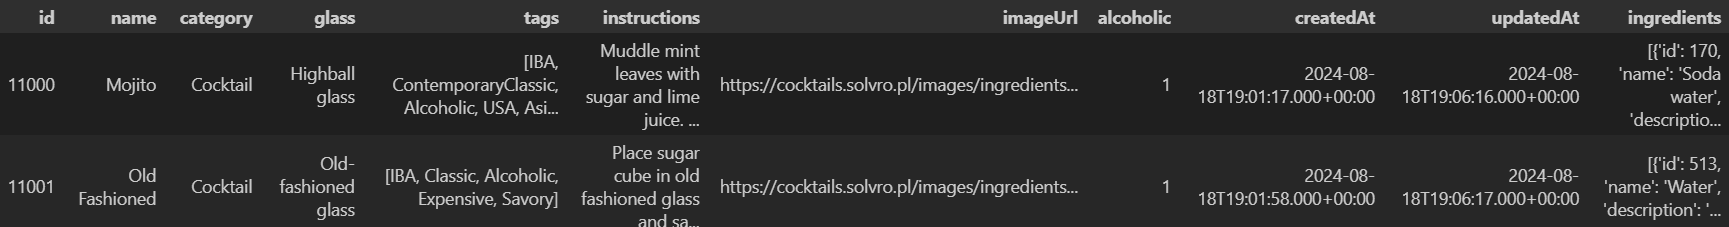
\includegraphics[width=1\linewidth]{base_head.png}
    \caption{TheCocktailDB head}
    \label{fig:TheCocktailDB_head}
\end{figure}

The columns are: id, name, category, glass, tags, instructions, imageUrl, alcoholic, createdAt, updatedAt, ingredients. Every column excpet 'id' and 'alcoholic' have object type. Other two are represented as int64.

In 'ingredients' column there is nested information about ingredients. Each drink have own piece of ingredients information there. If you unpack such block of information there will be data about ingredients needed to prepare such drink. Every record in 'ingredients' table has 10 attributes. They are as follows: id, name, alcohol, type, percentage, imageUrl, createdAt, updatedAt, measure. After unpacking ingredients data from every cocktail there will be \textbf{531} unique records in the 'ingredients' table.

\begin{figure}[H]
    \centering
    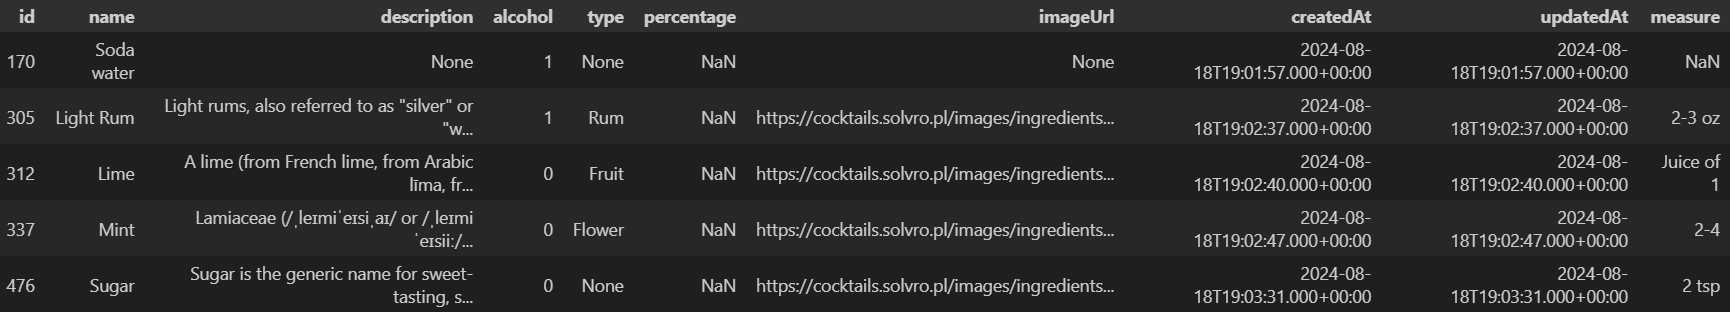
\includegraphics[width=1\linewidth]{ingredients_head.png}
    \caption{A snippet of the 'ingredients' table}
    \label{fig:ingredients_head}
\end{figure}

\section{Data review}
\subsection{Data loading}
In this section, we will demonstrate the steps required to load the dataset into our analysis environment. As we found out data is stored in .json format, so loading it into pandas DataFrame looks like this:
\begin{figure}[H]
    \centering
    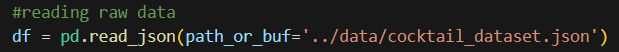
\includegraphics[width=1\linewidth]{loading.png}
    \caption{Loading data and storing it as pandas DataFrame}
    \label{fig:enter-label}
\end{figure}

\subsection{Missing values}
In this section we will examine missing values in our DataFrame and correct type of data in time columns. Figure 4 represents summed rows of missing values in each column of the dataset. We can see that most of the 'tags' column is missing (\textbf{99 out of 134}). Figure 5 shows code used to correct data type in 'createdAt' and 'updatedAt' columns.
\vspace{2cm}

\begin{multicols}{2}

\begin{figure}[H]
    \centering
    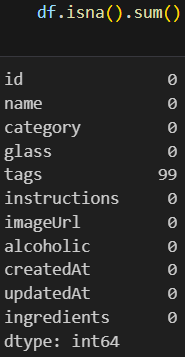
\includegraphics[width=0.4\linewidth]{types.png}
    \caption{Sums on missing values}
    \label{fig:enter-label}
\end{figure}

\columnbreak

\begin{figure}[H]
    \centering
    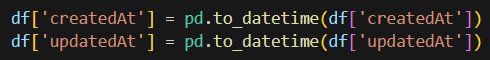
\includegraphics[width=1\linewidth]{type correction.png}
    \caption{Data type correction}
    \label{fig:enter-label}
\end{figure}

\end{multicols}

\subsection{Brief exploration}
After short reconnaissance of the data in our DataFrame you can spot some important properties:
\begin{itemize}
    \item every cocktail is alcoholic
    \item imageUrl won't be useful in the data analysis (at least for us)
    \item id's aren't consistent
    \item 'ingredients' column is stuffed with a .json data
\end{itemize}
In that case further explorations of the dataset will exclude 'imageUrl' and 'alcoholic' columns.

\section{Exploring cocktails alone}
In this section we pay attention only to cocktails - we won't unpack data from 'ingredients' column. In this case we drop four columns: 'ingredients', 'imageUrl', 'alcoholic', 'tags'.
\subsection{Is there something hidden in those times?}
Creating and updating times may seem harmless and boring but is there something hidden? Let's plot them and find out! Figure 6 shows the result, seems that nothing interesting was hidden there. Next we will simplify a little and assume that length of the instruction is somehow relevant to level of preparation complexity. We will replace textual value of instructions with the length of it. Below (on Figure 7) you can see brief code and the results of such operation. In this case we can, for example, find relations between type of the glass and the instruction length. Figure 8 presents lenghts of the instruction per every type of glass. Each red dot represents one cocktail. We can spot that Highball glasses tend to have a little longer instructions than Cocktail glasses. Old-fashioned glass drinks' instruction length vary more than Cocktails glass ones which are more regular.
\vspace{4cm}

\begin{figure}[H]
    \centering
    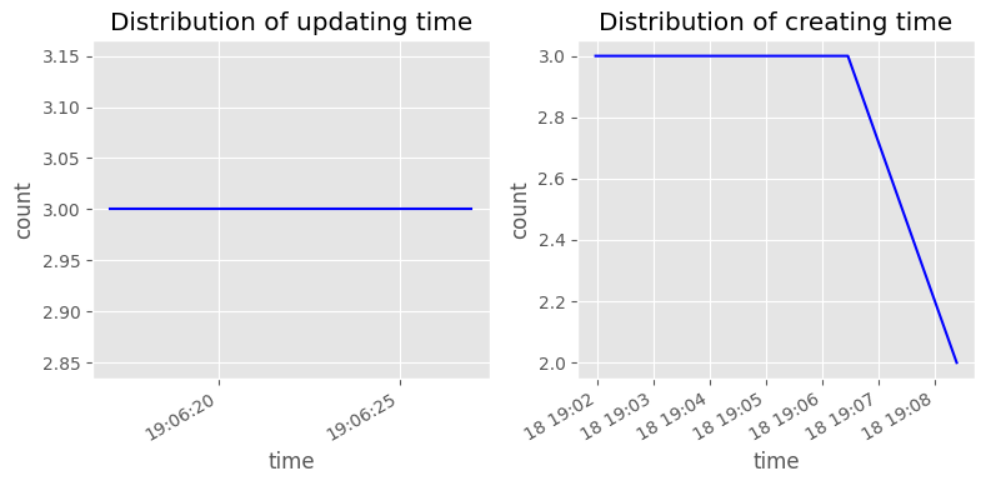
\includegraphics[width=0.8\linewidth]{times cocktails.png}
    \caption{Times of creating and upgrading cocktails}
    \label{fig:enter-label}
\end{figure}

\begin{figure}[H]
    \centering
    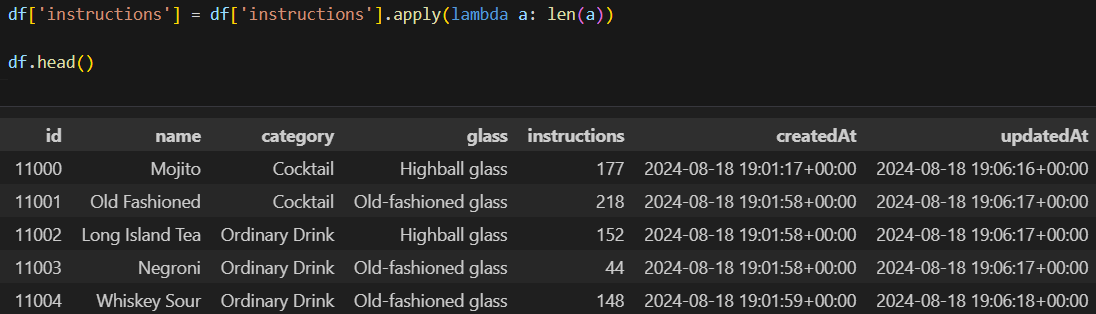
\includegraphics[width=1\linewidth]{simplify.png}
    \caption{Replacement of the instruction and  current look at head of our cocktails data}
    \label{fig:enter-label}
\end{figure}

\begin{figure}[H]
    \centering
    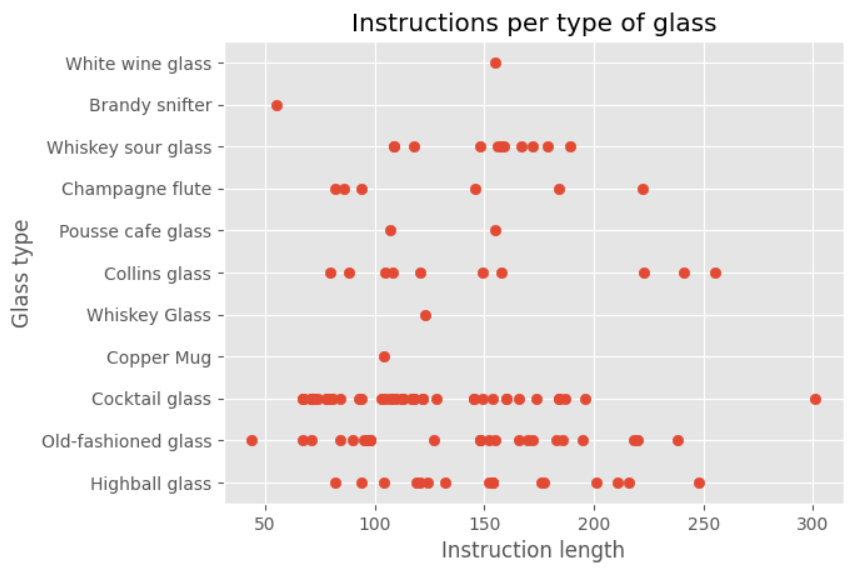
\includegraphics[width=0.8\linewidth]{ins length.png}
    \caption{Length of the instruction per type of the glass}
    \label{fig:enter-label}
\end{figure}

\subsection{Dividing into groups}
Let's take a look at popularity of each drink category. There are three such categories: Punch / Party Drink, Cocktail, Ordinary Drink. To count how many drinks are in each category we will use function: value\_counts(), then we will simply plot it as horizontal bar plot. Here is the result (Figure 9):

\begin{figure}[H]
    \centering
    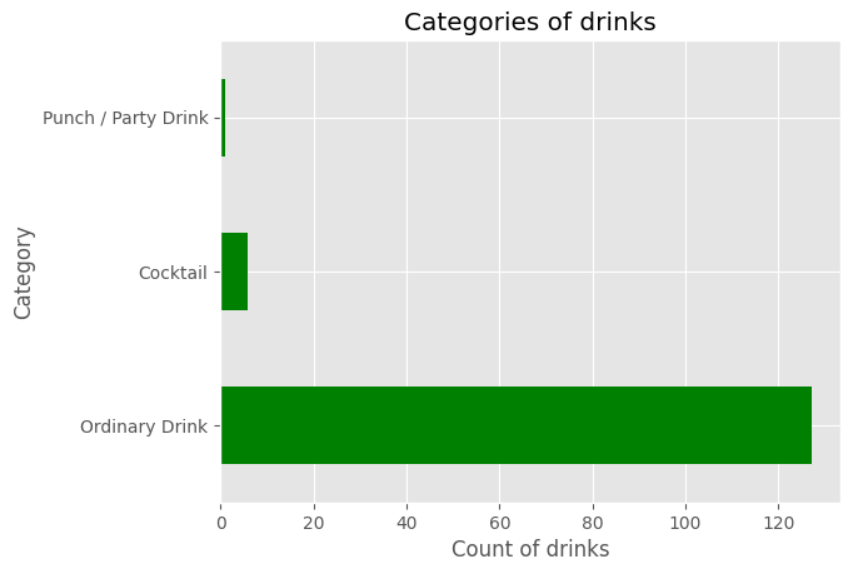
\includegraphics[width=0.7\linewidth]{categories.png}
    \caption{Count of drinks in each category}
    \label{fig:enter-label}
\end{figure}

Similarly we can count the frequency of using each glass type in drinks and present the mon bar plot. This time we will focus on top 10 used glass types.

\begin{figure}[H]
    \centering
    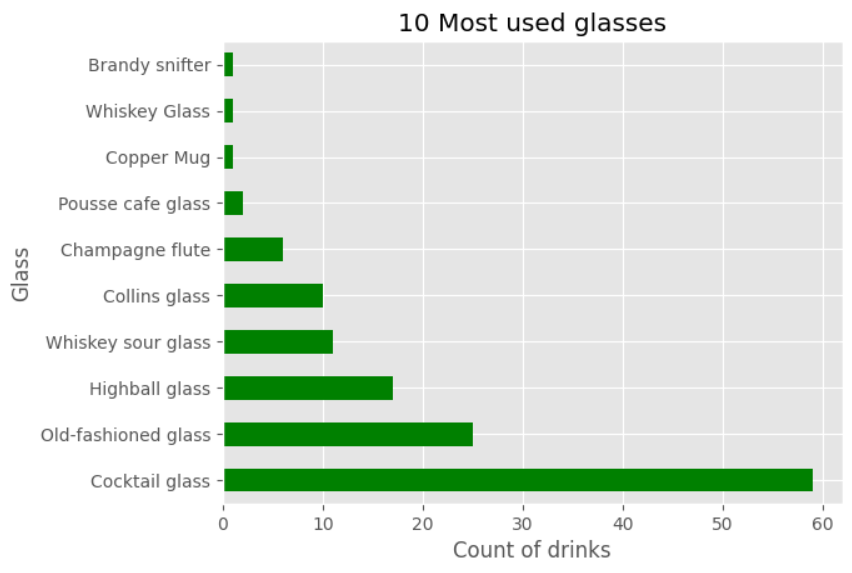
\includegraphics[width=0.9\linewidth]{glass types.png}
    \caption{Top 10 used glasses}
    \label{fig:enter-label}
\end{figure}

As we can see most commonly used glass type is Cocktail glass, second one is Old-fashioned glass and on third position there is Highball glass. The top one leaves opponents far behind.



\end{document}